%%%%%%%%%%%%%%%%%%%%%%%%%%%%%%%%%%%%%%%%%%%%%%%%%%%%%%%%%%%%%%%%%%%%%%%%%%%%%%%%
%2345678901234567890123456789012345678901234567890123456789012345678901234567890
%        1         2         3         4         5         6         7         8

\documentclass[letterpaper, 10 pt, conference]{ieeeconf}  % Comment this line out if you need a4paper

%\documentclass[a4paper, 10pt, conference]{ieeeconf}      % Use this line for a4 paper

\IEEEoverridecommandlockouts                              % This command is only needed if 
                                                          % you want to use the \thanks command

\overrideIEEEmargins                                      % Needed to meet printer requirements.

% See the \addtolength command later in the file to balance the column lengths
% on the last page of the document

% The following packages can be found on http:\\www.ctan.org
%\usepackage{graphics} % for pdf, bitmapped graphics files
%\usepackage{epsfig} % for postscript graphics files
%\usepackage{mathptmx} % assumes new font selection scheme installed
%\usepackage{times} % assumes new font selection scheme installed
%\usepackage{amsmath} % assumes amsmath package installed
%\usepackage{amssymb}  % assumes amsmath package installed



\usepackage{amsmath,amssymb}
\usepackage{tikz,hyperref,graphicx,units,subfig}
\usepackage{sidecap,wrapfig}
\usepackage[ruled,vlined]{algorithm2e}
\DeclareMathOperator*{\argmin}{arg\,min}
\DeclareMathOperator*{\argmax}{arg\,max}
\newcommand{\abs}[1]{\lvert#1\rvert} 
\newcommand{\norm}[1]{\lVert#1\rVert}
%\newcommand{\suchthat}{\mid}
\newcommand{\suchthat}{\ \big|\ }
\newcommand{\bd}{\mathbf{d}}
\newcommand{\bn}{\mathbf{n}}
\newcommand{\bp}{\mathbf{p}}
\newcommand{\bw}{\mathbf{w}}
\newcommand{\by}{\mathbf{y}}
\newcommand{\bx}{\mathbf{x}}
\newcommand{\bz}{\mathbf{z}}
\newcommand{\bbf}{\mathbf{f}}
\newcommand{\bzero}{\mathbf{0}}
\newcommand{\bG}{\mathbf{G}}
\newcommand{\bA}{\mathbf{A}}
\newcommand{\bW}{\mathbf{W}}
\newcommand{\bX}{\mathbf{X}}
\newcommand{\mX}{\mathcal{X}}
\newcommand{\mD}{\mathcal{D}}
\newcommand{\mN}{\mathcal{N}}
\newcommand{\mW}{\mathcal{W}}
\newcommand{\mF}{\mathcal{F}}
\newcommand{\bZ}{\mathbf{Z}}

\newcommand{\bfc}{W}
\newcommand{\Qinf}{Q_{\infty}}
\newcommand{\st}[1]{_\text{#1}}
\newcommand{\rres}{r\st{res}}
\newcommand{\pos}[1]{(#1)^+}
\newcommand{\depth}{\operatorname{depth}}
\newcommand{\dist}{\operatorname{dist}}
\newcommand{\convhull}{\operatorname{ConvexHull}}
\newcommand{\minksum}{\operatorname{MinkowskiSum}}



\title{\LARGE \bf
Grasp Metric for Gaussian Proccess Implicit Surface Representation of Shape Uncertainity }


\author{Michael Laskey,Zoe McCarthy, Sachin Patil, Pieter Abbeel and Ken Goldberg}% <-this % stops a space



\begin{document}



\maketitle
\thispagestyle{empty}
\pagestyle{empty}


%%%%%%%%%%%%%%%%%%%%%%%%%%%%%%%%%%%%%%%%%%%%%%%%%%%%%%%%%%%%%%%%%%%%%%%%%%%%%%%%
\begin{abstract}

This electronic document is a �live� template. The various components of your paper [title, text, heads, etc.] are already defined on the style sheet, as illustrated by the portions given in this document.

\end{abstract}


%%%%%%%%%%%%%%%%%%%%%%%%%%%%%%%%%%%%%%%%%%%%%%%%%%%%%%%%%%%%%%%%%%%%%%%%%%%%%%%%
\section{Introduction}

\vspace{10pt}
\noindent{\textbf{Grasp Quality Metrics}}: A number of metrics have been proposed to evaluate form and force closure with scalar quality measures for grasping \cite{bicchi2000}. We use the wrench-space Ferrari-Canny force closure quality measures \cite{ferrari1992}, which aims to maximize the disturbance that can be resisted given bounds on the contact forces. We also consider the general case where there is friction at the contact points. We follow the analysis of Schulman et al. \cite{schulman2011} in the discussion below.\\


\noindent{\textbf{Gaussian Process (GP) Primer}}: Gaussian processes (GPs) are widely used in machine learning as a nonparametric regression method for estimating continuous functions from sparse and noisy data \cite{rasmussen2006}. In a GP, a training set consists of input vectors $\mX = \{\bx_1, \ldots, \bx_n\}, ~\bx_i \in \mathbb{R}^d$, and corresponding observations $\by = \{y_1, \ldots, y_n\}$. The observations are assumed to be noisy measurements from the unknown target function $f$:
\begin{equation}
y_i = f(\bx_i) + \epsilon,
\end{equation}
where $\epsilon \sim \mN(0,\sigma^2)$ is Gaussian noise in the observations. A zero-mean Gaussian process is completely specified by a covariance function $k(\cdot,\cdot)$, also referred to as a kernel. Given the training data $\mD = \{\mX, \by\}$ and covariance function $k(\cdot,\cdot)$, the posterior density $p(f_*|\bx_*,\mD)$ at a test point $\bx_{*}$ is shown to be \cite{rasmussen2006}:
\begin{equation}
p(f_*|\bx_*,\mD) \sim \mN\big(k(\mX,\bx_*)^{\intercal}(K + \sigma_{\epsilon}^2I)^{-1}\by, k(\bx_*,\bx_*)-k(\mX,\bx_*)^{\intercal}(K+\sigma^2I)^{-1}k(\mX,\bx_*)\big), \label{eq:GPposterior}
\end{equation}
where $K \in \mathbb{R}^{n \times n}$ is a matrix with entries $K_{ij} = k(\bx_i,\bx_j)$ and $k(\mX,\bx_*) = [k(\bx_1,\bx_*),\ldots,k(\bx_n,\bx_*)]^{\intercal}$. 

The choice of kernel is application-specific, since the function $k(\bx_i,\bx_j)$ is used as a measure of correlation between states $\bx_i$ and $\bx_j$. A common choice is the squared exponential kernel:
\begin{equation}
k(\bx_i,\bx_j) = \nu^2\exp(-\frac{1}{2}(\bx_i - \bx_j)^{\intercal}\Lambda^{-1}(\bx_i - \bx_j))
\end{equation}
where $\Lambda= \text{diag}(\lambda_1^2,\ldots,\lambda_d^2)$ are the characteristic length scales of each dimension of $\bx$ and $\nu^2$ describes the variability of $f$. The vector of hyper-parameters $\boldsymbol{\theta} = \{\sigma,\nu,\lambda_1,\ldots,\lambda_d\}$ is chosen or optimized during the training process by minimizing the log likelihood $p(\by|\mX,\boldsymbol{\theta})$ \cite{rasmussen2006}.

\section{Related Work}

\section{Problem Definition}
Given a grasp $G$ on an object, we can define it by the following tuple $G = \lbrace c_1,...,c_m,n_1,...,n_m,z,\mu\rbrace$. We have a set $I$ of $m$ contacts on the object where $i \in I$ contact is located at $c_i$ with surface normal $n_i$. The object has a center of mass $z$ and friction coefficient $\mu$. We demonstrate that one can efficiently compute a close form distribution for $c_i$,$n_i$ and $z$. We note though that our metric assumes a given $\mu$. \\

 For the following derivations we use the following notation. $\theta(x) = \lbrace \mu(x),\Sigma(x) \rbrace$, hence $\theta(x)$ is a tuple consisting of the mean and covariance functions given by the trained GPIS. We further assume that the contacts on the gripper approach along a line of action: $x = \gamma(t): R \rightarrow R^n$. The line segment has endpoints $a,b$ that are defined as the start of the gripper and end of the voxel grid respectively, as shown in Fig. \ref{fig:line_of_action}.We also denote the level set function as $f(x): \mathbb{R}^N \rightarrow \mathbb{R}$ 

\begin{figure}[ht!]
\centering
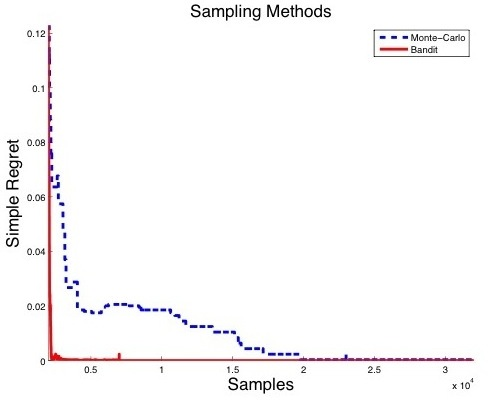
\includegraphics[scale = 0.3]{figures/Slide1.jpg}
\caption{Parameterized Line of Action along a Object}
\vspace*{-10pt}
\label{fig:line_of_action}
\end{figure}


\section{Distribution of Grasp Parameters}


\subsection{Distribution on Contact Points}: The probability along the line $\gamma(g)$ is given by the following:

\begin{equation}
P(f(\gamma(g))|\theta(\gamma(g))) = N(\mu_T,\Sigma_T)
\end{equation}

This gives the distributions along the entire line of action, however we want to compute the marginalization of this where at each point we simply are asking the probability $p(f(\gamma(g=k))=0)$. We can achieve this by marginalizing out the rest of the points along the line. With a Gaussian it has the closed form solution as follows: 

\begin{equation}
P(c_{i,det} =  P(f(\gamma(g))=0|\theta(\gamma(t)))
\end{equation}


\subsection{Distribution on Surface Normals} The distribution of surface normals $P(n_i = k)$ can be calculate as follows. First we assume that some function exists $h(x) = \lbrace \mu_{\nabla}(x), \Sigma_{\nabla}(x) \rbrace$, hence given a point $x$ it returns the parameters for a Gaussian distribution around the gradient. this function can be computed via learning the gradient \cite{gradient} or analytical differentiation of $f(x)$. We note though that both methods yields a Gaussian distribution. We now demonstrate how to marginalize out the contact distribution and compute $P(n_i = k)$\\

From our distribution on contact points and Bayes rule we can compute the following: 

\begin{equation}
p(c_i = \gamma{g}, n_i = k) = p(n_i = k | h(\gamma{g}))*p(c_i = \gamma{g})
\end{equation}

Now we can marginalize out the distribution on contacts:

\begin{equation}
P(n_i = k) = \int_T  p(n_i = k | h(\gamma{g}))*p(c_i = \gamma{g}) dg
\end{equation}

Which over the voxel grid turns into: 

\begin{equation}
P(n_i = k) = \sum_T  p(n_i = k | h(\gamma{g}))*p(c_i = \gamma{g}) dg
\end{equation}


Thus, $P(n_i = k)$ is a multi-modal distributions  composed of Gaussians sum together. 

\subsection{Distribution on Center of Mass} Zoe fill out or we all die :-(


\subsection{Other Thoughs Not Finished}
The derivation above assumes that the robot doesn't have any noise in its movements. To accomdate noise in the position of the gripper at time $t$, $x_t$ given control input $u_{t}$ and previous states $x_{1:t-1}$, we introduce the following probability $P(x_t=k|u_t,x_{1:t-1})$. This can be computed by methods like an Extended Kalman Filter (EKF) or a particle filter. For simplicity we assume that it is a Guassian distribution. 

We know derive the following: 

\begin{equation}
P(c_{i}) = \int P(c_{i,det}=\gamma(g),x_t = \gamma(g)) dg
\end{equation}

\section{Probabilistic Bound on Grasp Metric}

\end{document}
